\documentclass[12pt]{article}
\usepackage{../template}

\graphicspath{ {./img/} }
\addbibresource{../references.bib}

\makeglossaries
\loadglsentries{../glossaries}

\begin{document}
    \glsresetall  % Reset first occurrences

    \subfile{covers/first_page.tex}

    \newpage
    \vspace{10em}
    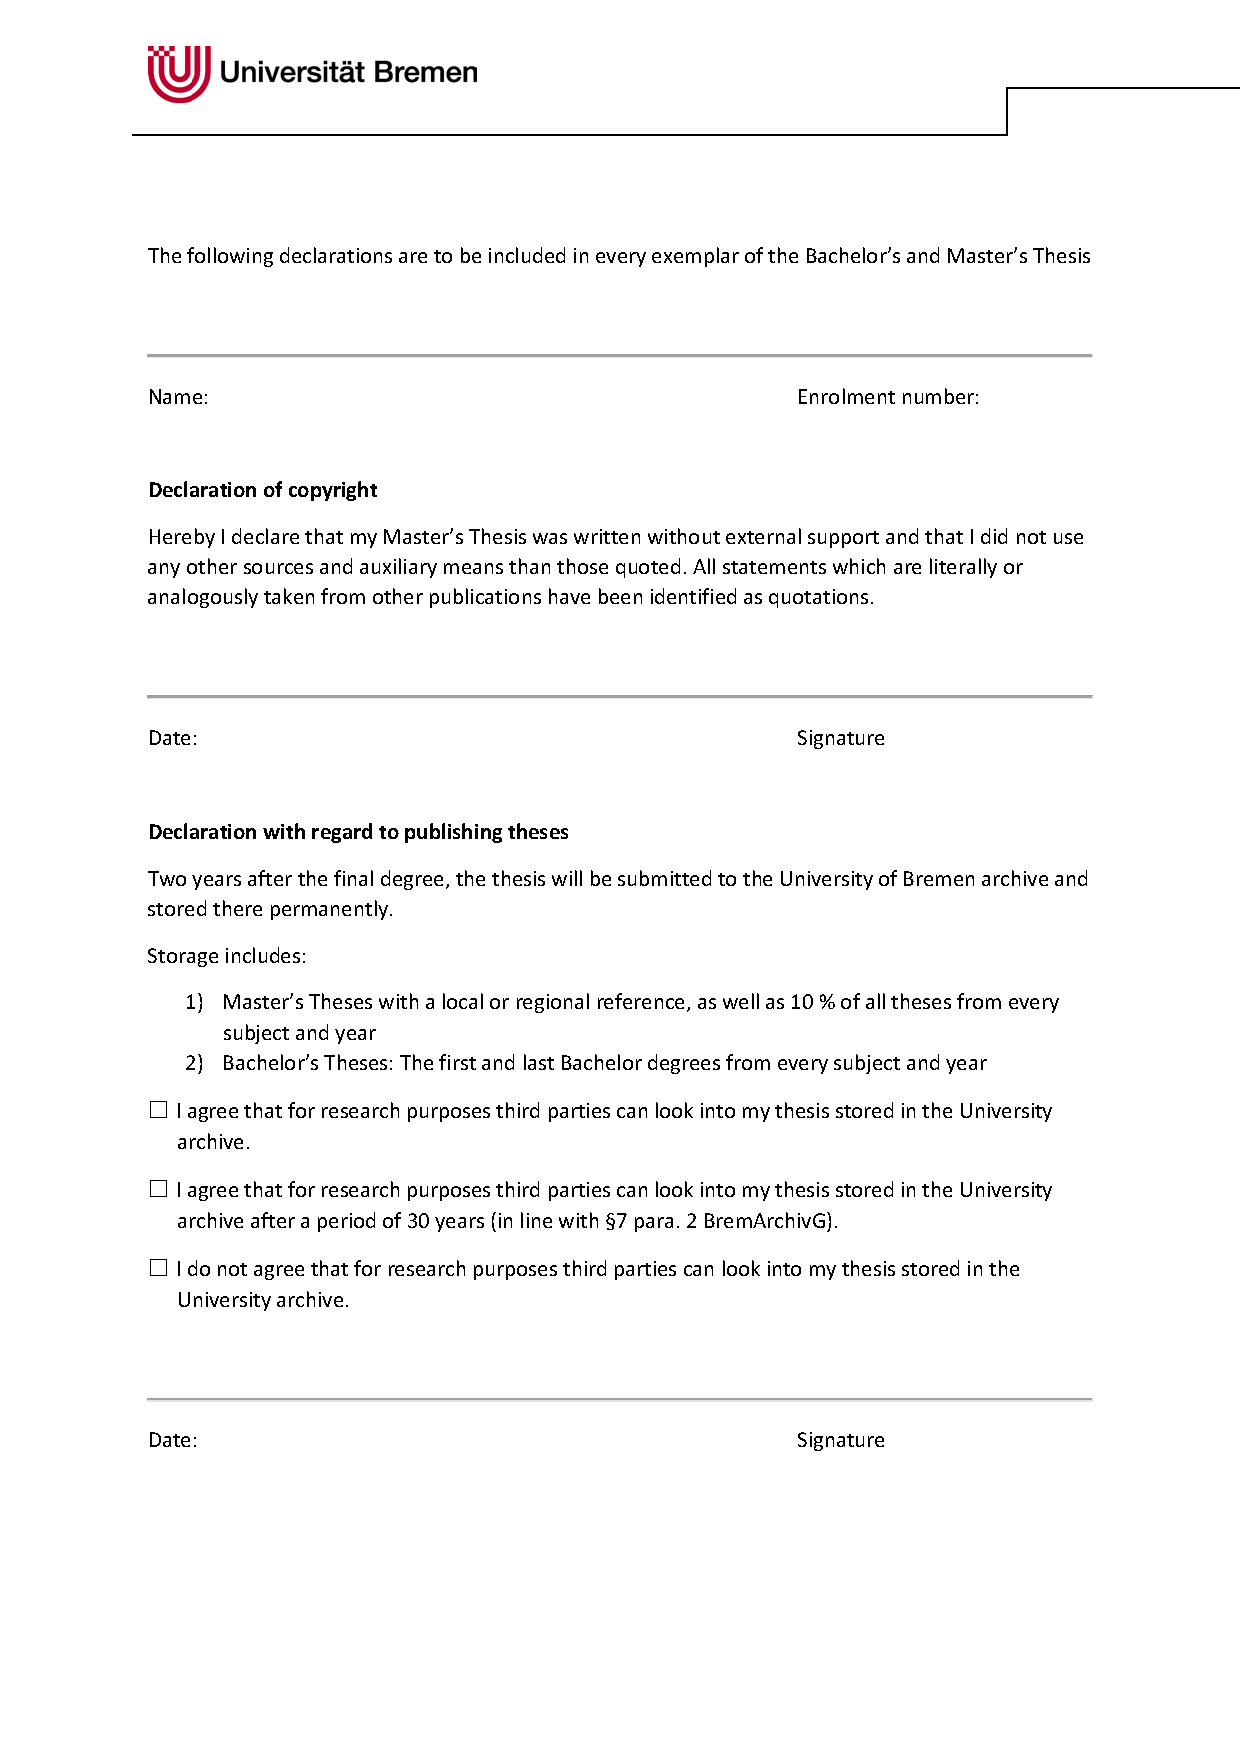
\includepdf[offset=-5mm -2cm]{./img/misc/Eigenstaendigkeitserklaerung_Master.pdf}

    \newpage
    \subfile{chapters/0_1_acknowledgments.tex}

    \newpage
    \subfile{chapters/0_2_abstract.tex}

    \newpage
    \tableofcontents

    \newpage
    \listoffigures

    \newpage
    \listoftables

    \newpage
    \printglossary[type=acronym]

    \newpage
    \subfile{./chapters/1_introduction.tex}
    \FloatBarrier

    \newpage
    \subfile{./chapters/2_materials_and_methods.tex}
    \FloatBarrier

    \newpage
    \subfile{./chapters/3_bio_backg_and_exp_motiv.tex}
    \FloatBarrier

    \newpage
    \subfile{./chapters/4_math_background.tex}
    \FloatBarrier

    \newpage
    \subfile{./chapters/5_0_results.tex}
    \FloatBarrier
    
    \newpage
    \subfile{chapters/discussion.tex}
    \FloatBarrier
    
    \appendix

    \newpage
    \subfile{appendices/a_additional_figures.tex}

    \newpage
    \subfile{appendices/b_model_parameters.tex}

    \newpage
    \subfile{appendices/c_scaling_noise_for_r5_and_helicon_cells.tex}

    \newpage
    \subfile{appendices/d_neuprint_dataset.tex}

    \newpage
    \printbibliography

\end{document}